%!TEX root = ../main.tex
%---------------------------------------------------------------------------------------------------
\FloatBarrier\section{Eckstein-Keane-Wolpin models}\label{Setting}
%---------------------------------------------------------------------------------------------------
We now present the general structure of Eckstein-Keane-Wolpin (EKW) models \citep{Aguirregabiria.2010}  and their solution approach. We then turn to the customized version used by \citet{Keane.1997} to study the career decisions of young men and investigate the consequences of parametric uncertainty in this empirically-grounded and computationally demanding setting. We outline their model's basic setup, provide some descriptive statistics of the empirical data used in our estimation, and then discuss the core findings.
%---------------------------------------------------------------------------------------------------
%---------------------------------------------------------------------------------------------------
\subsection{General structure}
%---------------------------------------------------------------------------------------------------
%---------------------------------------------------------------------------------------------------
EKW models describe sequential decision-making under uncertainty \citep{Gilboa.2009, Machina.2014}. At time $t = 1, \hdots, T$ each individual observes the state of their choice environment $s_t\in S$ and chooses an action $a_t$ from the set of admissible actions $\mathcal{A}$. The decision has two consequences: an individual receives an immediate utility $u_t(s_t, a_t)$ and their environment evolves to a new state $s_{t + 1}$. The transition from $s_t$ to $s_{t + 1}$ is affected by the action but remains uncertain. Since individuals are forward-looking, they do not simply choose the alternative with the highest immediate utility. Instead, they take the future consequences of their actions into account.\\

\noindent A policy $\pi =(d^\pi_1, \hdots, d^\pi_T)$ provides the individual with instructions for choosing an action in any possible future state. It is a sequence of decision rules $d^\pi_t$ that specify the action $d^\pi_t(s_t) \in \mathcal{A}$   at a particular time $t$ for any possible state $s_t$ under $\pi$. The implementation of a policy generates a sequence of utilities that depends on the objective transition probability distribution $p_t(s_t, a_t)$ for the evolution from state $s_t$ to $s_{t + 1}$ induced by the model.\\

\noindent Figure \ref{Timing} depicts the timing of events for two generic periods.  At the beginning of period $t$, an individual fully learns about each action's immediate utility, selects one of the alternatives, and receives its immediate utility. Then, the state evolves from $s_t$ to $s_{t + 1}$, and the process repeats itself in $t + 1$.\\

\begin{figure}\centering
%!TEX root = ../main.tex
% \definecolor{gray}{RGB}{31,119,180}

% \definecolor{light-gray}{gray}{0.85}


\begin{tikzpicture}[node distance=2cm]
%define styles
\tikzstyle{startstop} = [circle, rounded corners, minimum width=0.6cm, minimum height=0.3cm,text centered, draw=black]
[
->,
>=stealth',
auto,node distance=3cm,
thick,
main node/.style={circle, draw, font=\sffamily\Large\bfseries}
]
\tikzstyle{arrow} = [thick,->,>=stealth]]
\tikzstyle{darrow} = [dotted,->,>=stealth]]
%first and second column

\node (r0) [startstop, xshift = -3cm, draw = none] {};
\node (r999) [startstop, xshift = 13cm, draw = none] {};

\node (r1) [startstop, xshift = -1cm] {\footnotesize $~\,s_t\,~$};
\node (r2) [startstop, xshift = 5cm] {\footnotesize $s_{t+1}$};  %previously 4
\node (r3) [startstop, xshift = 11cm] {\footnotesize $s_{t+2}$}; %previously 8

\draw [arrow, dashed] (r0) -- node[anchor=south] {} (r1) ;
\draw [arrow] (r1) -- node[anchor=south] {} (r2) ;
\draw [arrow] (r2) -- node[anchor=south] {} (r3) ;
\draw [arrow, dashed] (r3) -- node[anchor=south] {} (r999) ;
t
\node (r4) [startstop, xshift = 0 cm, yshift = -2.5cm, inner sep = 0.08cm] {\footnotesize $~\,a_t\,~$ };
\node (r5) [startstop, xshift = 3.5
 cm, yshift = -2.5cm, inner sep = 0.08cm] {\footnotesize $~\,u_t\,~$ };
\node (r6) [startstop, xshift = 6 cm, yshift = -2.5cm, inner sep = 0.08cm] {\footnotesize $a_{t+1}$ };
\node (r7) [startstop, xshift = 9.5 cm, yshift = -2.5cm, inner sep = 0.08cm] {\footnotesize $u_{t+1}$ };

\draw [arrow] (r1) -- node[anchor=south] {} (r4) ;
\draw [arrow] (r2) -- node[anchor=south] {} (r6) ;

\draw[ thick](0,-2.05).. controls (0.75, -0.2) and (0.8,0)..(1.5, 0);
\draw [arrow] (r4) -- node[anchor=south] {} (r5) ;
\draw[ thick](6,-2.05).. controls (6.75, -0.2) and (6.85,0)..(7.5, 0);
\draw [arrow] (r6) -- node[anchor=south] {} (r7) ;


\node(r8)[startstop, xshift = - 1.3cm, yshift = -1.3cm, draw =none, align=center] {\footnotesize decide \\ \footnotesize $d_t^{\pi}(s_t)$ };
\node(r9)[startstop, xshift= 4.6cm, yshift = -1.3cm, draw =none, align = center] {\footnotesize decide \\ \footnotesize $d_{t+1}^{\pi}(s_{t+1})$ };
\node(r10)[startstop, yshift = 1cm, xshift = 2cm, draw =none, align=center ] {\footnotesize transition \\ \footnotesize $p_t(s_t, a_t)$};
\node(r11)[startstop, yshift = 1cm, xshift = 8cm, draw =none, align=center ] { \footnotesize transition \\ \footnotesize $p_{t+1}(s_{t+1}, a_{t+1})$};
%\node(r10)[startstop, yshift = 0.5cm, xshift = 1.7cm, draw =none, align=center ] {\footnotesize transition \\ \footnotesize $p(s_t, a_t)$};
%\node(r11)[startstop, yshift = 0.5cm, xshift = 8cm, draw =none, align=center ] {\footnotesize transition \\ \footnotesize $p(s_{t+1}, a_{t+1})$};
\node(r12)[startstop, yshift = -2cm, xshift = 1.7cm, draw =none, align=center ] {\footnotesize receive\\ \footnotesize $u_t(s_t, a_t)$};
\node(r13)[startstop, yshift = -2cm, xshift = 7.7cm, draw =none, align=center ] {\footnotesize receive\\ \footnotesize $u_{t+1}(s_{t+1}, a_{t+1})$};

\end{tikzpicture}

\caption{Timing of events}\label{Timing}
\end{figure}

\noindent Individuals make their decisions facing uncertainty about the future and seek to maximize their expected total discounted utilities over all decision periods given all available information. They have rational expectations \citep{Muth.1961}, so their subjective beliefs about the future agree with the objective probabilities for all possible future events provided by the model. Immediate utilities are separable between periods \citep{Kahneman.1997}, and a discount factor $\delta$ parameterizes a preference for immediate over future utilities \citep{Samuelson.1937}.\\

\noindent Equation (\ref{Objective Risk}) formally describes the individual's objective. Given an initial state $s_1$, they implement a policy $\pi$ that maximizes the expected total discounted utilities over all decision periods given the information available at the time.
%
\begin{align}\label{Objective Risk}
\max_{\pi \in \Pi} \E_{s_1}^\pi\left[\,\sum^{T}_{t = 1}  \delta^{t - 1} u_t(s_t, d^\pi_t(s_t))\,\right]
\end{align}

\noindent EKW models are set up as a standard Markov decision process (MDP) \citep{Puterman.1994,Rust.1994,White.1993} that can be solved by a simple backward induction procedure. In the final period $T$, there is no future to consider, and the optimal action is choosing the alternative with the highest immediate utility in each state. With the decision rule for the final period, we can determine all other optimal decisions recursively. We use our group's open-source research code \verb+respy+ \citep{Gabler.2020b}, which allows for the flexible specification, simulation, and estimation of EKW models. Detailed documentation of the software and its numerical components is available at \url{http://respy.readthedocs.io}.
%---------------------------------------------------------------------------------------------------
%---------------------------------------------------------------------------------------------------
\subsection{The career decisions of young men}
%---------------------------------------------------------------------------------------------------
%---------------------------------------------------------------------------------------------------
\citet{Keane.1997} specialize the model above to explore the career decisions of young men regarding their schooling, work, and occupational choices using the National Longitudinal Survey of Youth 1979 (NLSY79) \citep{NLSY.2019} for the estimation of the model. We restrict ourselves to a basic summary of their setup. Further documentation of the model specification and the observed dataset is available in the Appendix.\\

\noindent \citet{Keane.1997} follows individuals over their working life from young adulthood at age 16 to retirement at age 65. Each decision period $t = 16, \dots, 65$ represents a school year. Figure \ref{Decision tree} illustrates the initial decision problem as individuals select one of five alternatives from the set of admissible actions $a\in\mathcal{A}$. They can  decide to either work in a blue-collar or a white-collar occupation ($a = 1, 2$), serve in the military $(a = 3)$, attend school $(a = 4)$, or stay at home $(a = 5)$.\\


\begin{figure}[t!]\centering
	\scalebox{0.75}{% Decision tree black white

\tikzset{
	treenode/.style = {shape=rectangle, rounded corners, draw, align=center, bottom color=blue!20},
	root/.style     = {treenode, font=\small, draw=none},
	env/.style      = {treenode, font=\small, draw=none},
	dummy/.style    = {circle,draw}
}


\begin{tikzpicture}
[
	x=30pt,
	y=26pt,
	yscale=-1,
	xscale=1,
	baseline=-120pt,
	grow                    = right,
	edge from parent/.style = {draw, -latex},
	every node/.style       = {font=\footnotesize, minimum width={width("Magnetometer")+2pt}},
	sloped
]


% Zero  level: START
\node [root, top color = white, bottom color=white, draw] (0) at (-10,0) {\textbf{Start}};


% First level: BLUE
\node [env, top color = bwtabblue, bottom color = bwtabblue, color = bwtaborange, scale = 0.8] (1) at (-5,-4.2) {\textbf{Blue}};
\draw[->, thick] (0) edge node[left of = 0, rotate = 72.75, node distance = 0.3cm]{} (1);
% Second level: Blue, White, Military, School, Home
\node [env, top color = bwtabblue, bottom color = bwtabblue, color = bwtaborange, scale = 0.55] (11) at (0,-5) {Blue};
\draw[->] (1) edge (11);
\node [env, top color = bwtabred, bottom color = bwtabred, color = bwtaborange, scale = 0.55] (12) at (0,-4.6) {White};
\draw[->] (1) edge (12);
\node [env, top color = bwtabpurple, bottom color = bwtabpurple, scale = 0.55] (13) at (0,-4.2) {Military};
\draw[->] (1) edge (13);
\node [env, top color = bwtaborange, bottom color = bwtaborange, scale = 0.55] (14)  at (0,-3.8) {School};
\draw[->] (1) edge (14);
\node [env, top color = bwtabgreen, bottom color = bwtabgreen, scale = 0.55] (15)  at (0,-3.4) {Home};
\draw[->] (1) edge (15);
% Third level coordinates
\coordinate (a1) at (3,-5);
\draw [->, dashed, color=tabgrey] (11) to[right] node[auto] {} (a1);
\coordinate (a2) at (3,-4.6);
\draw [->, dashed, color=tabgrey] (12) to[right] node[auto] {} (a2);
\coordinate (a3) at (3,-4.2);
\draw [->, dashed, color=tabgrey] (13) to[right] node[auto] {} (a3);
\coordinate (a4) at (3,-3.8);
\draw [->, dashed, color=tabgrey] (14) to[right] node[auto] {} (a4);
\coordinate (a5) at (3,-3.4);
\draw [->, dashed, color=tabgrey] (15) to[right] node[auto] {} (a5);



%First level: WHITE
\node [env, top color = bwtabred, bottom color = bwtabred, color = bwtaborange, scale=0.8] (2) at (-5,-2.1) {\textbf{White}};
\draw[->, thick] (0) edge node[right of = 0, yshift=0.35cm,  rotate = 41.0, node distance = 0cm]{} (2);
% Second level: Blue, White, Military, School, Home
\node [env, top color = bwtabblue, bottom color = bwtabblue, color = bwtaborange, scale = 0.55] (21) at (0,-2.9) {Blue};
\draw[->] (2) edge (21);
\node [env, top color = bwtabred, bottom color = bwtabred, color = bwtaborange, scale = 0.55] (22) at (0,-2.5) {White};
\draw[->] (2) edge (22);
\node [env, top color = bwtabpurple, bottom color = bwtabpurple, scale = 0.55] (23) at (0,-2.1) {Military};
\draw[->] (2) edge (23);
\node [env, top color = bwtaborange, bottom color = bwtaborange, scale = 0.55] (24)  at (0,-1.7) {School};
\draw[->] (2) edge (24);
\node [env, top color = bwtabgreen, bottom color = bwtabgreen, scale = 0.55] (25)  at (0,-1.3) {Home};
\draw[->] (2) edge (25);
% Second level --> third level
\coordinate (e1) at (3,-2.9);
\draw [->, dashed, color = tabgrey] (21) to[right] node[auto] {} (e1);
\coordinate (e2) at (3,-2.5);
\draw [->, dashed, color = tabgrey] (22) to[right] node[auto] {} (e2);
\coordinate (e3) at (3,-2.1);
\draw [->, dashed, color = tabgrey] (23) to[right] node[auto] {} (e3);
\coordinate (e4) at (3,-1.7);
\draw [->, dashed, color = tabgrey] (24) to[right] node[auto] {} (e4);
\coordinate (e5) at (3,-1.3);
\draw [->, dashed, color = tabgrey] (25) to[right] node[auto] {} (e5);


% First Level: MILITARY
\node [env, top color = bwtabpurple, bottom color = bwtabpurple, scale = 0.8] (3) at (-5,0) {\textbf{Military}};
\draw[->, thick] (0) edge node[right of = 0, yshift = 0.25cm, node distance = 0.2cm]{} (3);
% Second level: Blue, White, Military, School, Home
\node [env, top color = bwtabblue, bottom color = bwtabblue, color = bwtaborange, scale = 0.55] (31) at (0,-0.8) {Blue};
\draw[->] (3) edge (31);
\node [env, top color = bwtabred, bottom color = bwtabred, color = bwtaborange, scale = 0.55] (32) at (0,-0.4) {White};
\draw[->] (3) edge (32);
\node [env, top color = bwtabpurple, bottom color = bwtabpurple, scale = 0.55] (33) at (0,0) {Military};
\draw[->] (3) edge (33);
\node [env, top color = bwtaborange, bottom color = bwtaborange, scale = 0.55] (34)  at (0,0.4) {School};
\draw[->] (3) edge (34);
\node [env, top color = bwtabgreen, bottom color = bwtabgreen, scale = 0.55] (35)  at (0,0.8) {Home};
\draw[->] (3) edge (35);
% Second level --> third level
\coordinate (c1) at (3,-0.8);
\draw [->, dashed, color = tabgrey] (31) to[right] node[auto] {} (c1);
\coordinate (c2) at (3,-0.4);
\draw [->, dashed, color = tabgrey] (32) to[right] node[auto] {} (c2);
\coordinate (c3) at (3,0);
\draw [->, dashed, color = tabgrey] (33) to[right] node[auto] {} (c3);
\coordinate (c4) at (3,0.4);
\draw [->, dashed, color = tabgrey] (34) to[right] node[auto] {} (c4);
\coordinate (c5) at (3,0.8);
\draw [->, dashed, color = tabgrey] (35) to[right] node[auto] {} (c5);


% First Level: SCHOOL
\node [env, top color = bwtaborange, bottom color = bwtaborange, scale = 0.8] (4)  at (-5,2.1) {\textbf{School}};
\draw[->, thick] (0) edge node[right of = 0, yshift=0.1cm, rotate = -38, node distance = 0.25cm]{} (4);
% Second level: Blue, White, Military, School, Home
\node [env, top color = bwtabblue, bottom color=bwtabblue, color = bwtaborange, scale = 0.55] (41) at (0,1.3) {Blue};
\draw[->] (4) edge (41);
\node [env, top color = bwtabred, bottom color=bwtabred, color = bwtaborange, scale = 0.55] (42) at (0,1.7) {White};
\draw[->] (4) edge (42);
\node [env, top color = bwtabpurple, bottom color=bwtabpurple, scale = 0.55] (43) at (0,2.1) {Military};
\draw[->] (4) edge (43);
\node [env, top color = bwtaborange, bottom color=bwtaborange, scale = 0.55] (44)  at (0,2.5) {School};
\draw[->] (4) edge (44);
\node [env, top color = bwtabgreen, bottom color=bwtabgreen, scale = 0.55] (45)  at (0,2.9) {Home};
\draw[->] (4) edge (45);
% Second level --> third level
\coordinate (b1) at (3,1.3);
\draw [->, dashed, color = tabgrey] (41) to[right] node[auto] {} (b1);
\coordinate (b2) at (3,1.7);
\draw [->, dashed, color = tabgrey] (42) to[right] node[auto] {} (b2);
\coordinate (b3) at (3,2.1);
\draw [->, dashed, color = tabgrey] (43) to[right] node[auto] {} (b3);
\coordinate (b4) at (3,2.5);
\draw [->, dashed, color = tabgrey] (44) to[right] node[auto] {} (b4);
\coordinate (b5) at (3,2.9);
\draw [->, dashed, color = tabgrey] (45) to[right] node[auto] {} (b5);


% First Level: HOME
\node [env, top color = bwtabgreen, bottom color = bwtabgreen, scale=0.8] (5)  at (-5,4.2) {\textbf{Home}};
\draw[->, thick] (0) edge node[right of = 0, yshift=0.25cm, rotate = -72.75, node distance = 0.15cm]{} (5);
%\draw[->, thick] (0) edge (5);
% Second level: Blue, White, Military, School, Home
\node [env, top color = bwtabblue, bottom color = bwtabblue, color = bwtaborange, scale = 0.55] (51)  at (0,3.4) {Blue};
\draw[->] (5) edge (51);
\node [env, top color = bwtabred, bottom color = bwtabred, color = bwtaborange, scale = 0.55] (52)  at (0,3.8) {White};
\draw[->] (5) edge (52);
\node [env, top color = bwtabpurple, bottom color = bwtabpurple, scale = 0.55] (53) at (0,4.2) {Military};
\draw[->] (5) edge (53);
\node [env, top color = bwtaborange, bottom color = bwtaborange, scale = 0.55] (54) at (0,4.6) {School};
\draw[->] (5) edge (54);
\node [env, top color = bwtabgreen, bottom color = bwtabgreen, scale=0.55] (55) at (0,5.0) {Home};
\draw[->] (5) edge (55);
% Second level --> third level
\coordinate (d1) at (3,3.4);
\draw [->, dashed, color = tabgrey] (51) to[right] node[auto] {} (d1);
\coordinate (d2) at (3,3.8);
\draw [->, dashed, color = tabgrey] (52) to[right] node[auto] {} (d2);
\coordinate (d3) at (3,4.2);
\draw [->, dashed, color = tabgrey] (53) to[right] node[auto] {} (d3);
\coordinate (d4) at (3,4.6);
\draw [->, dashed, color = tabgrey] (54) to[right] node[auto] {} (d4);
\coordinate (d5) at (3,5.0);
\draw [->, dashed, color = tabgrey] (55) to[right] node[auto] {} (d5);

\end{tikzpicture}

\vspace{1cm}
}
	\caption{Decision tree}\label{Decision tree}
\end{figure}\FloatBarrier

\noindent Individuals are already heterogeneous when entering the model. They differ with respect to their level of initial schooling $h_{16}$, and have one of four different $\mathcal{J} = \{1, \hdots, 4\}$ alternative-specific skill endowment types $\bm{e} = \left(e_{j,a}\right)_{\mathcal{J} \times \mathcal{A}}$.\\

\noindent The immediate utility $u_a(\cdot)$ of each alternative consists of a non-pecuniary utility $\zeta_a(\cdot)$ and, at least for the working alternatives, an additional wage component $w_a(\cdot)$. Both depend on the level of human capital as measured by their alternative-specific skill endowment $\bm{e}$, their years of completed schooling $h_t$, and their occupation-specific work experience $\bm{k_t} = \left(k_{a,t}\right)_{a\in\{1, 2, 3\}}$. The immediate utilities are influenced by last-period choices $a_{t -1}$ and alternative-specific productivity shocks $\bm{\epsilon_t} = \left(\epsilon_{a,t}\right)_{a\in\mathcal{A}}$ as well. Their general form is given by:
%
\begin{align*}
u_a(\cdot) =
\begin{cases}
    \zeta_a(\bm{k_t}, h_t, t, a_{t -1})  + w_a(\bm{k_t}, h_t, t, a_{t -1}, e_{j, a}, \epsilon_{a,t})                & \text{if}\, a \in \{1, 2, 3\}  \\
    \zeta_a(\bm{k_t}, h_t, t, a_{t-1}, e_{j,a}, \epsilon_{a,t})                                                  &  \text{if}\, a \in \{4, 5\}.
\end{cases}
\end{align*}
%
\noindent Work experience $\bm{k_t}$  and years of completed schooling $h_t$ evolve deterministically. There is no uncertainty about grade completion \citep{Altonji.1993} and no part-time enrollment. Schooling is defined by time spent in school, not by formal credentials acquired. Once individuals reach a certain amount of schooling, they acquire a degree.
%
\begin{align*}
k_{a,t+1} = k_{a,t} + \ind[a_t = a]  &\qquad \text{if}\, a \in \{1, 2, 3\} \\
h_{t + 1\phantom{,a}} = h_{t\phantom{,a}} +   \ind[a_t = 4]  &\qquad
\end{align*}
%
\noindent The productivity shocks $\bm{\epsilon_t}$ are uncorrelated across time and follow a multivariate normal distribution with mean $\bm{0}$ and covariance matrix $\bm{\Sigma}$. Given the structure of the utility functions and the distribution of the shocks, the state at time $t$ is $s_t = \{\bm{k_t}, h_t, t, a_{t -1}, \bm{e},\bm{\epsilon_t}\}$.\\

\noindent Skill endowments $\bm{e}$ and initial schooling $h_{16}$ are the only sources of persistent heterogeneity in the model. All remaining differences in life-cycle decisions result from different transitory shocks $\bm{\epsilon_t}$ that occur over time.\\

\noindent Theoretical and empirical research from specialized disciplines within economics informs the specification of each $u_a(\cdot)$. As an example, we provide the exact functional form of the non-pecuniary utility from schooling in Equation (\ref{eq:UtilitySchoolingMain}). Further details on the specification of the utility functions are available in the Appendix.
%
\begin{align}\label{eq:UtilitySchoolingMain}
		\zeta_4(s_t)   = & \underbrace{e_{j,4}}_{\text{type}} + \underbrace{\beta_{tc_1} \cdot \ind[h_t \geq 12] + \beta_{tc_2} \cdot \ind[h_t \geq 16]}_{\text{tuition costs}}  + \underbrace{\gamma_{4,4} \cdot t + \gamma_{4,5} \cdot \ind[t < 18]}_{\text{time trend}}  \\[15pt]
	    							  & + \underbrace{\beta_{rc_1} \cdot \ind[a_{t-1} \neq 4, h_t < 12]   + \beta_{rc_2} \cdot \ind[a_{t-1} \neq 4, h_t \geq 12]}_{\text{re-enrollment cost}}  + \hdots + \epsilon_{4,t}\nonumber
\end{align}
%
There is a direct cost in the form of tuition for continuing education after high school $\beta_{tc_1}$ and college $\beta_{tc_2}$. The decision to leave school is reversible, but entails re-enrollment costs that differ by schooling category ($\beta_{rc_1}, \beta_{rc_2}$).\\

\noindent We analyze the original dataset used by \citet{Keane.1997}. We only provide a brief description and relegate further details to the Appendix. The authors construct their sample based on the NLSY79, a nationally representative sample of young men and women living in the United States in 1979 and born between 1957 and 1964. Individuals were followed from 1979 onwards and repeatedly interviewed about their schooling decisions and labor market experiences. Based on this information, individuals are assigned to either working in one of the three occupations, attending school, or simply staying at home.\\

\noindent \citet{Keane.1997} restrict attention to white men, who turned 16 between 1977 and 1981, and exploit information collected between 1979 and 1987. Thus, individuals in the sample range in age between 16 and 26 years old. While the sample initially consists of 1,373 individuals at age 16, this number drops to 256 at the age of 26 due to sample attrition and missing data. Overall, the final sample consists of 12,359 person-period observations.\\

\noindent Figure \ref{Overview} summarizes the evolution of choices and wages over the sample period. Roughly 86\% of individuals initially enroll in school, but this share steadily declines with age. Nevertheless, about 39\% pursue some form of higher education and obtain more than a high school degree. As individuals leave school, most of them initially pursue a blue-collar occupation. However, the relative share of white-collar workers increases as individuals entering the labor market later gain access to higher levels of schooling. At age 26, about 48\% work in a blue-collar occupation and 34\% in a white-collar occupation. The share of individuals in the military peaks around age 20 at 8\%. At its maximum around age 18, approximately 20\% of individuals stay at home.\\

\begin{figure}[t!]\centering
\subfloat[Choices]{\scalebox{0.25}{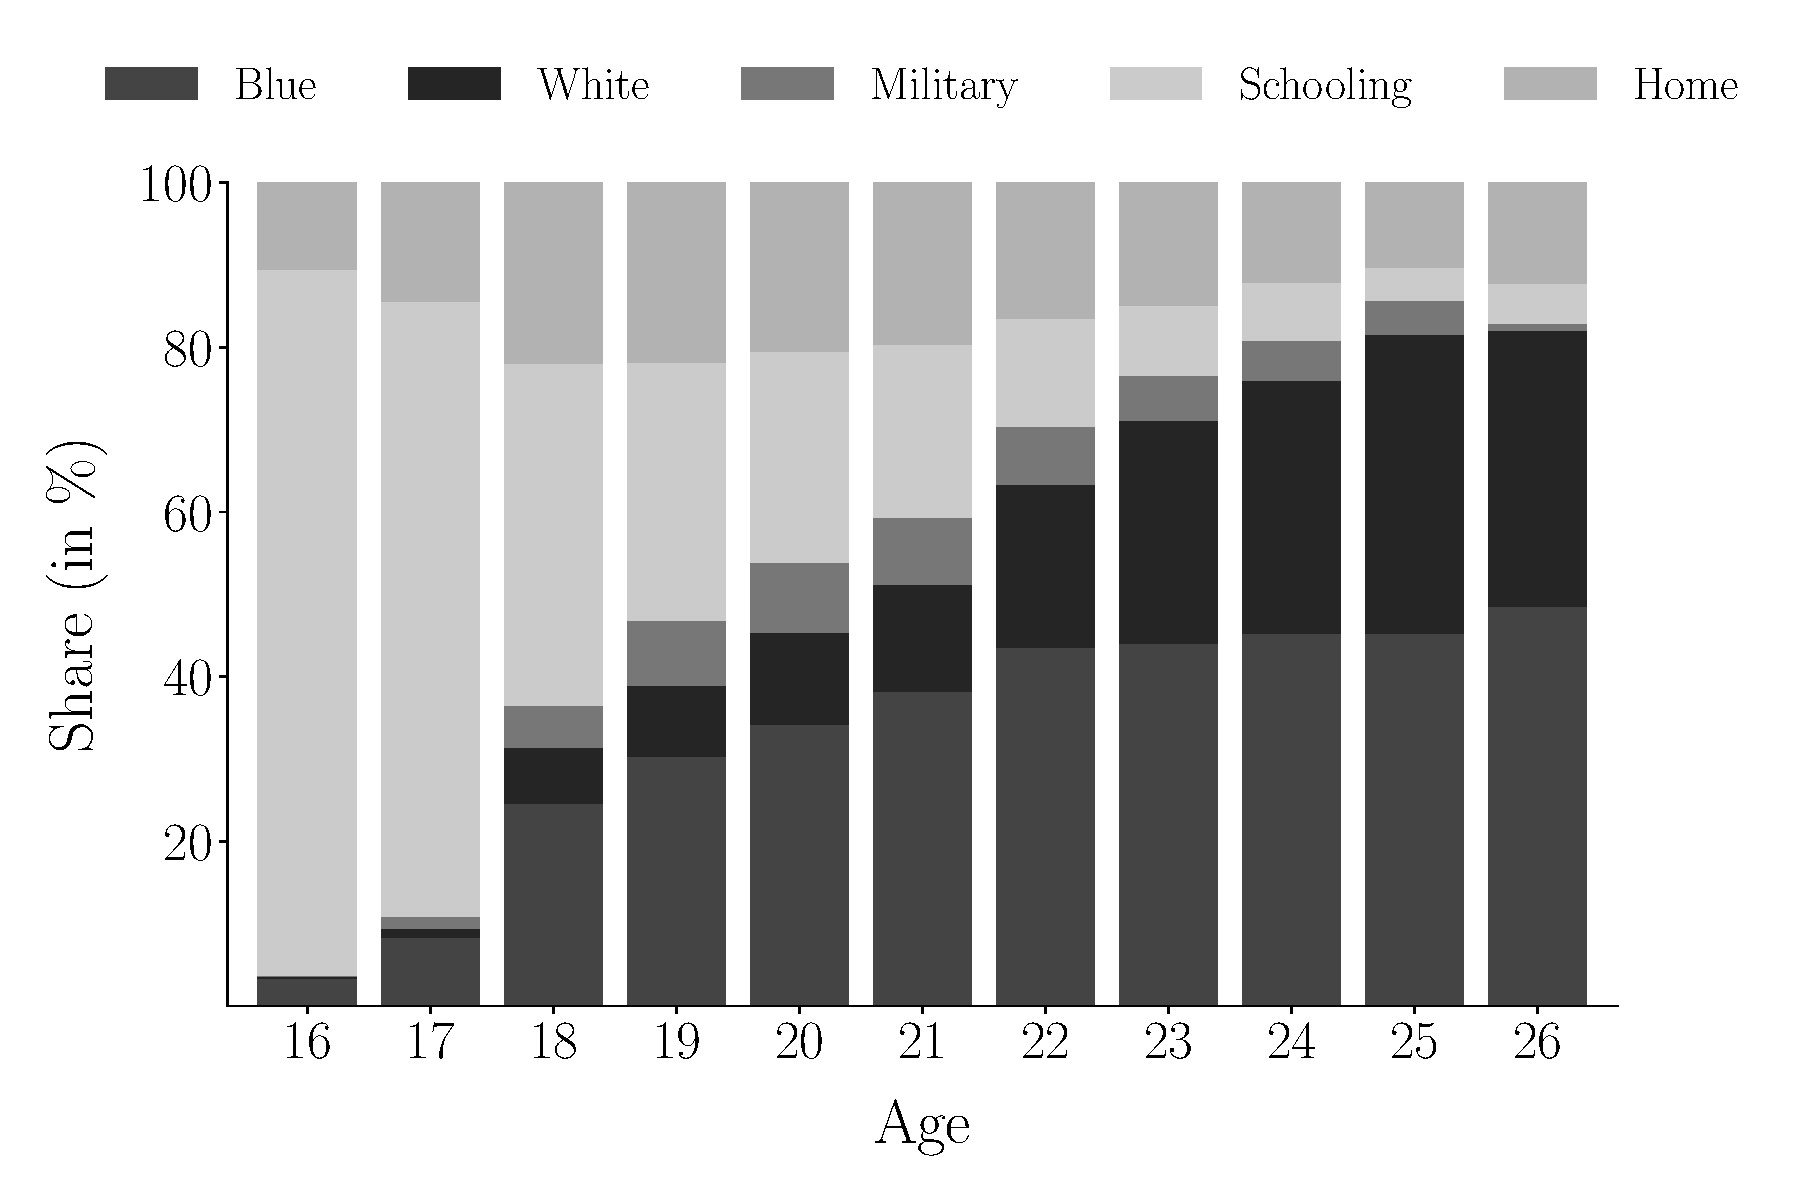
\includegraphics{fig-observed-data-choices-bw}}}\hspace{0.3cm}
\subfloat[Average wage]{\scalebox{0.25}{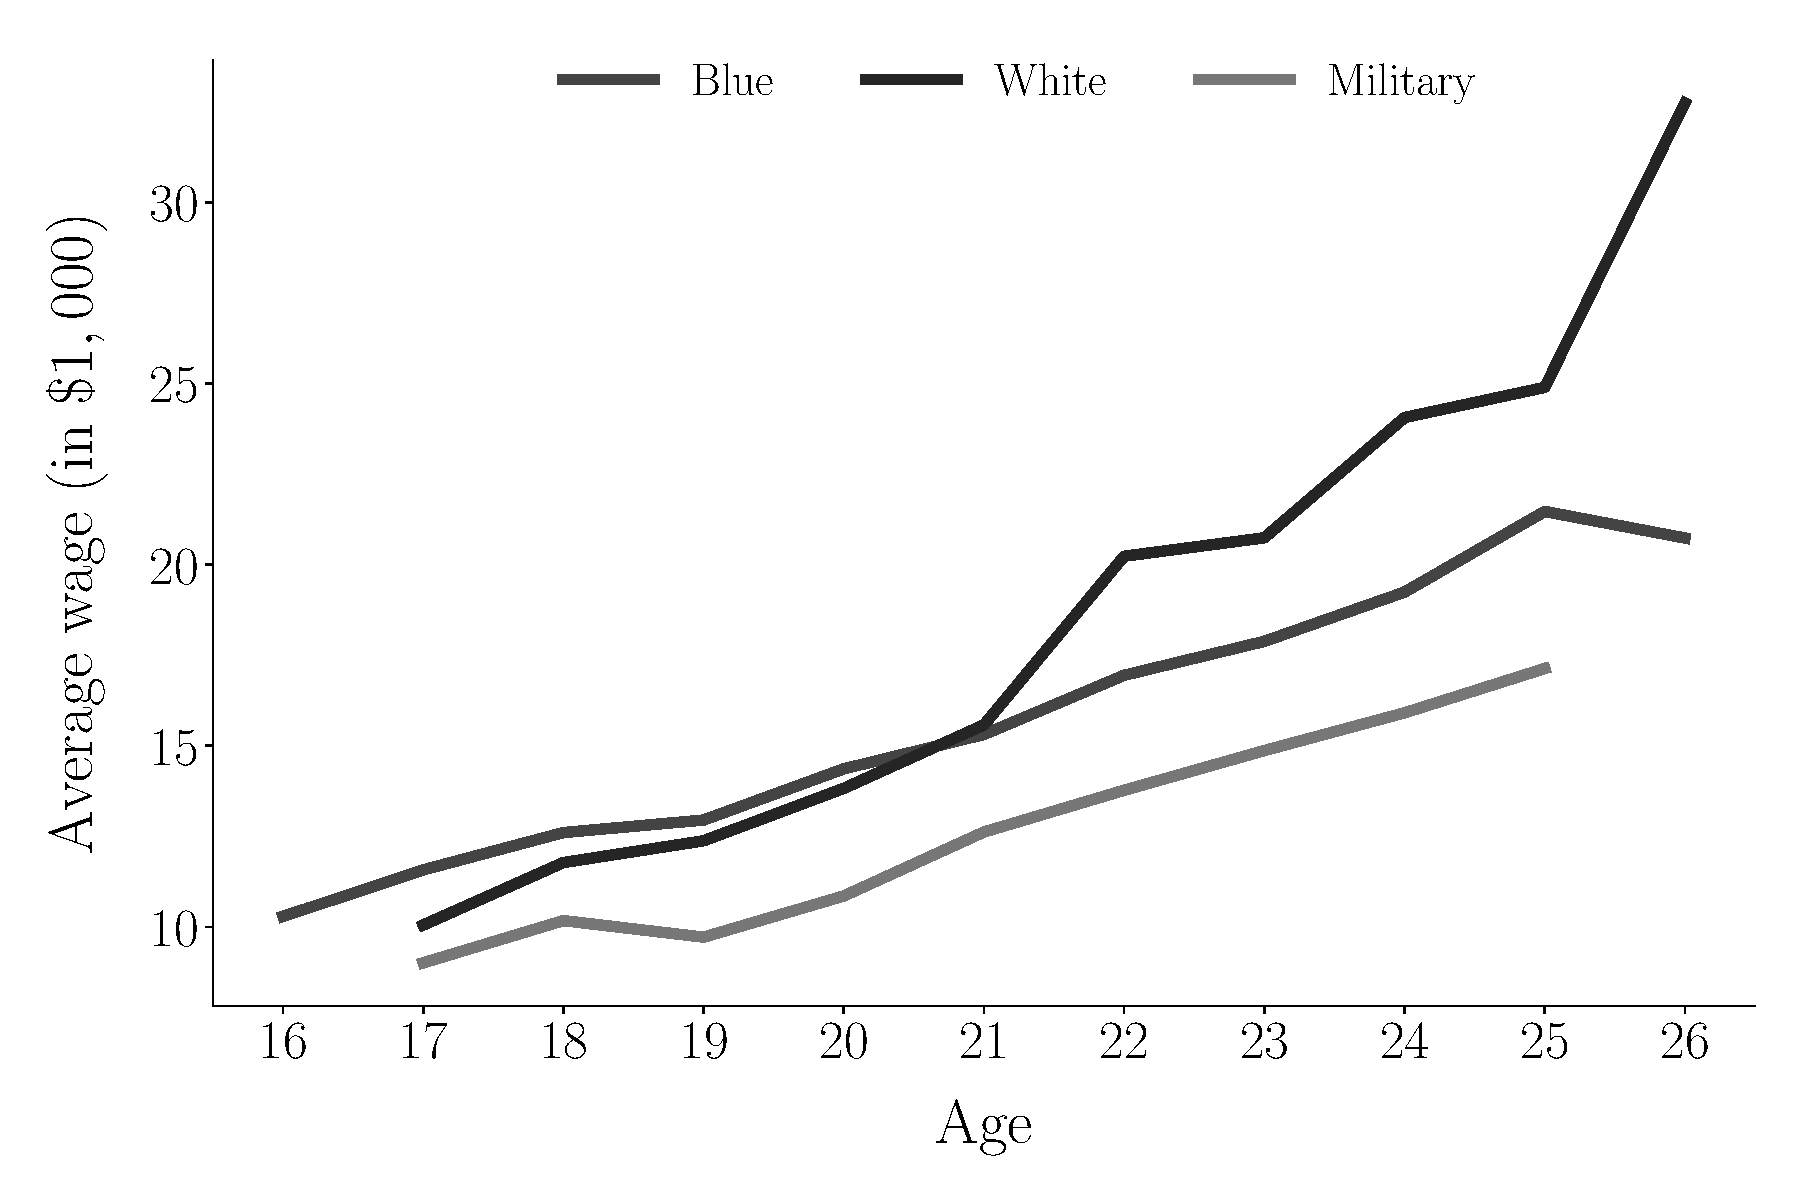
\includegraphics{fig-observed-wage-mean-bw}}}
\begin{center}
\begin{minipage}[t]{0.8\columnwidth}
\item \scriptsize{\textbf{Notes:} The wage is a full-time equivalent deflated by the gross national product deflator, with 1987 as the base year. We do not report the wage if less than ten observations are available.}
\end{minipage}
\end{center}
\caption{Data overview}\label{Overview}
\end{figure}\FloatBarrier

\noindent For an individual, the average wage starts at about \$10,000 at age 16 and increases considerably up to about \$25,000 by the age of 26. While starting wages for blue-collar workers are about \$10,286, wages in white-collar occupations and the military start around \$9,000. However, wages for white-collar occupations increase sharply over time, overtaking blue-collar wages around age 21. By the end of the observation period, wages for white-collar occupations are about 50\% higher than blue-collar wages at \$32,756 compared to only \$20,739. Military wages remain lowest throughout.\\

\noindent We consider observations for $i = 1, \hdots, N$ individuals in each time period $t = 1, \dots, T_i$. For every observation $(i, t)$ in the data, we observe the action $a_{it}$, some components $\bar{u}_{it}$ of the utility, and a subset $\bar{s}_{it}$ of the state $s_{it}$. Therefore, from an economist's point of view, we must distinguish between two types of state variables $s_{it} = \{\bar{s}_{it}, \bm{e},\bm{\epsilon_t}\}$. At time $t$, the economist and individual both observe $\bar{s}_{it}$, while $\{ \bm{e},\bm{\epsilon_t}\}$ is only observed by the individual.\\

\noindent We use  simulated maximum likelihood \citep{Fisher.1922,Manski.1977} estimation and determine the $88$ model parameters $\hat{\btheta}$ that maximize the likelihood function $\mathcal{L}(\btheta\mid\mathcal{D})$. As we only observe a subset $\bar{s}_t = \{\bm{k_t}, h_t, t, a_{t -1}\}$ of the state, we can determine the probability $p_{it}(a_{it}, \bar{u}_{it} \mid \bar{s}_{it}, \btheta)$ of individual $i$ at time $t$ in $\bar{s}_{it}$ choosing $a_{it}$ and receiving $\bar{u}_{it}$ given parametric assumptions about the distribution of $\bm{\epsilon_t}$. The objective function takes the following form:
%
\begin{align*}
  \hat{\btheta} \equiv \argmax_{\btheta \in \bTheta}  \underbrace{\prod^N_{i= 1} \prod^{T_i}_{t= 1}\, p_{it}(a_{it}, \bar{u}_{it} \mid \bar{s}_{it}, \btheta)}_{\mathcal{L}(\btheta\mid\mathcal{D})}.
\end{align*}
%
\noindent Overall, our parameter estimates are in broad agreement with the results reported in the original paper and the related literature. For example, individuals discount future utilities by $6\%$ per year. The returns to schooling vary according to occupation. While wages for white-collar occupations increase by about $6\%$ with each additional year of schooling, they only increase by $2\%$ for those working blue collar jobs. Skills are transferable across occupations as work experience increases wages in both blue and white-collar occupations.\\

\noindent Figure \ref{Model fit} shows the overall agreement between the empirical data and a dataset simulated using the estimated model parameters. We show average wages and the share of individuals choosing a blue-collar occupation over time. The results are based on a simulated sample of $10,000$ individuals. Additional model fit statistics are available in the Appendix.
%
\begin{figure}[h!]\centering
\subfloat[Average wage]{\scalebox{0.25}{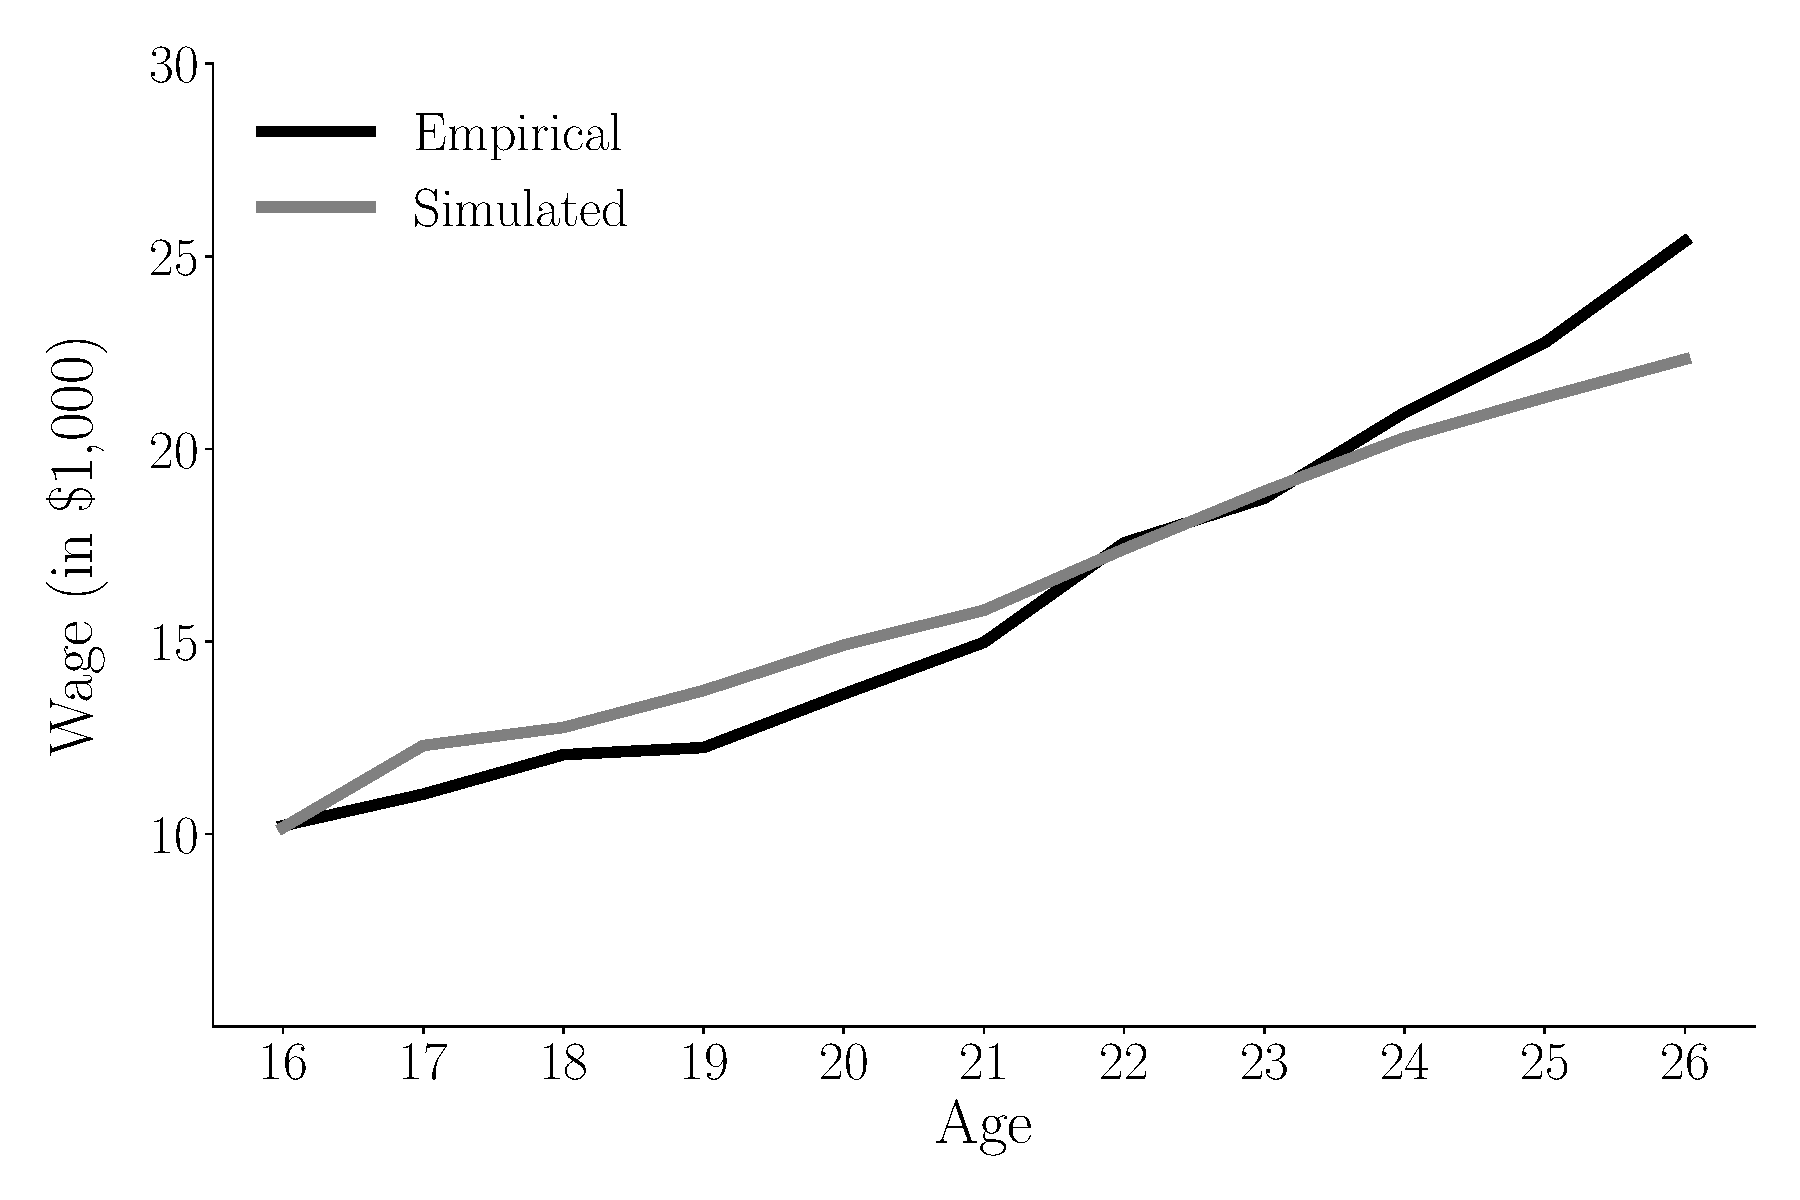
\includegraphics{fig-model-fit-wage-all-bw}}}
\subfloat[Blue-collar]{\scalebox{0.25}{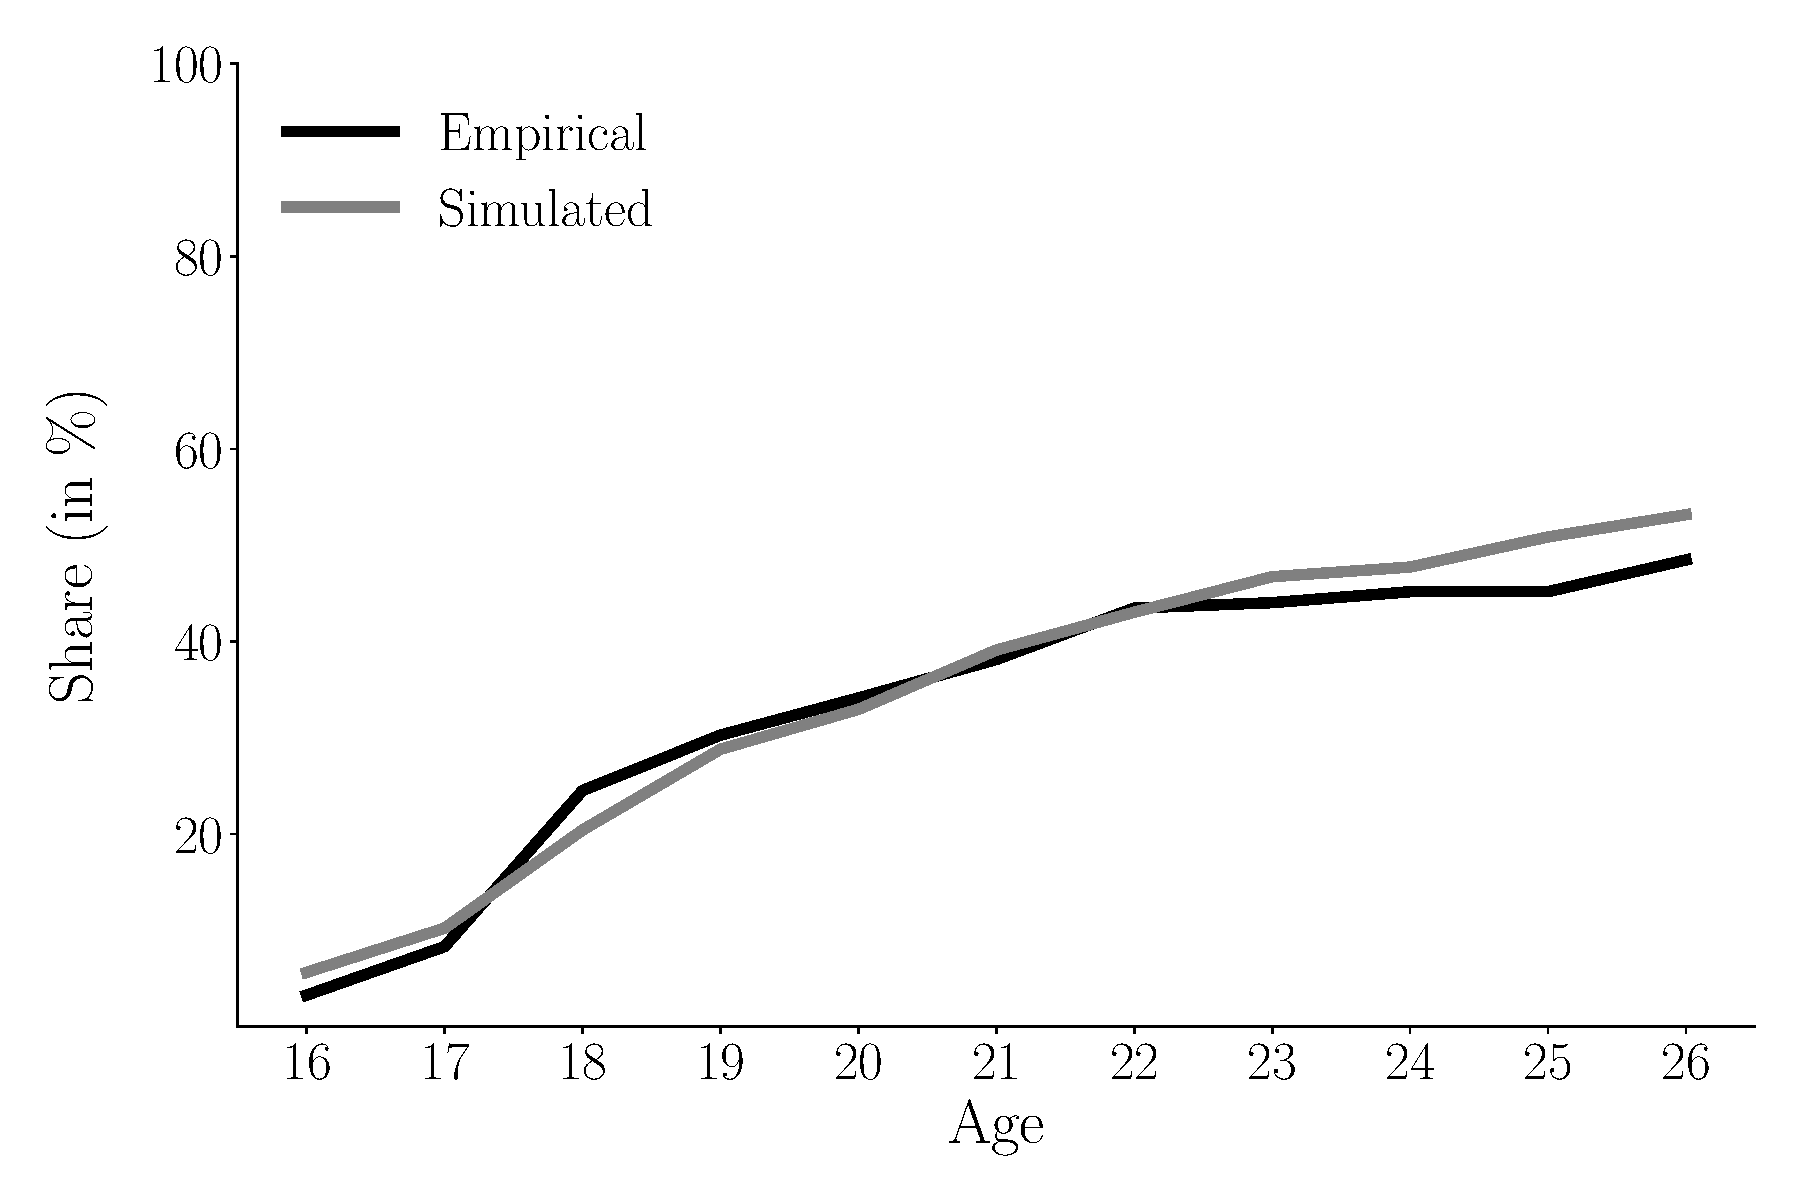
\includegraphics{fig-model-fit-choice-blue-bw}}}
\caption{Model fit}\label{Model fit}
\end{figure}\FloatBarrier

\noindent We adhere to the procedure outlined by the authors of the original paper and use the estimated model to conduct the ex-ante evaluation of a  $\$2,000$ tuition subsidy on educational attainment. We simulate a sample of  $10,000$ individuals using the point estimates and compare completed schooling to a sample of the same size, but with a reduction of $\hat{\beta}_{tc_1}$ by $\$2,000$. The subsidy increases average final schooling by 0.65 years. College graduation increases by 13 percentage points, and high school graduation rates improve by 4 percentage points.
%---------------------------------------------------------------------------------------------------
%---------------------------------------------------------------------------------------------------
\subsection{Confidence set bootstrap}
%---------------------------------------------------------------------------------------------------
%---------------------------------------------------------------------------------------------------
The construction of confidence sets for counterfactuals in many structural models poses two distinct challenges. First, the computational burden of even a single estimation of the model is considerable. This makes the application of a standard bootstrap approach \citep{Efron.1979} infeasible. Second, the nonlinear mapping from the parameters of the model to the counterfactual predictions often has kinks or is truncated. For example, in our case, the predicted impact of a tuition subsidy is bounded from below by zero. This violates the smoothness requirements of the delta method.\\

\noindent We use the Confidence Set (CS) bootstrap to construct the confidence set of the counterfactual. Although the CS bootstrap was originally proposed in \citet{Rao.1973}, it has only recently been formalized by \cite{Woutersen.2019}. Its application does not require repeated estimations of the model, as it uses the asymptotic normal distribution of the estimator for $\hat{\btheta}$. Furthermore, its validity does not depend on the differentiability of the prediction function.\footnote{See \citet{Reich.2020} for a critical assessment of confidence sets based on asymptotic arguments. They advocate the use of likelihood-ratio confidence intervals instead and set up their computation as a constraint optimization problem.}\\

\noindent Algorithm \ref{Confidence Set bootstrap} provides a concise description of the steps involved, where $\chi_l^2(1 - \alpha)$ is the quantile function for probability $1 - \alpha$ of the chi-square distribution with $l$ degrees of freedom.\\

\floatname{algorithm}{\sffamily\small Algorithm}
\begin{algorithm}[!th]
	\caption{\small\!\textbf{.\:\:}\textsf{\strut Confidence Set bootstrap}}\label{Confidence Set bootstrap}
	\begin{algorithmic}\vspace{0.3cm}

    \For{$m = 1, \hdots, M$}

    \State Draw $\hat{\btheta}_m \sim \N(\hat{\btheta}, \hat{\bs{\Sigma}})$

    \If{$(\hat{\btheta}_m - \hat{\btheta} )^\prime \hat{\Sigma}^{-1} (\hat{\btheta}_m - \hat{\btheta}) \leq \chi_l^2(1 - \alpha)$}
      \State Compute $\hat{y}_{g,m} = \M_g(\hat{\btheta}_m )$
			\State Add $\hat{y}_{g,m}$ to sample $Y=\{\hat{y}_{g,1}, \hdots, \hat{y}_{g,m-1}\}$
  \EndIf

		\EndFor
    \State Set $\Theta_{y_g}(\alpha) = [\min(Y), \max(Y)]$
		\vspace{0.3cm}\end{algorithmic}
\end{algorithm}\FloatBarrier

\noindent To summarize, we draw a large sample of $M$ parameters from the estimated asymptotic normal distribution of our estimator with mean $\hat{\btheta}$ and covariance matrix $\hat{\bs{\Sigma}}$, accepting only those draws that are elements of the confidence set of the model parameters. We then compute the counterfactual for all remaining draws and calculate the confidence set for the counterfactual based on its lowest and highest value.\\

\noindent The CS bootstrap poses a considerable computational challenge. In many applications, including our own, a single prediction of a counterfactual takes several minutes. At the same time, the number of parameter samples must be large to ensure that the minimum and maximum values for the counterfactual prediction are reliable. However, the algorithm is amenable to parallelization using modern high-performance computational resources by processing each of the $M$ parameter draws independently.\\

\noindent Our uncertainty sets then take the following form:
%
\begin{align*}\begin{array}{ll}
\U(\alpha) & \equiv\,\,  \left\{\btheta \in\bTheta: (\btheta - \hat{\btheta} )^\prime \hat{\Sigma}^{-1} (\btheta - \hat{\btheta}) \leq \chi_l^2(1 - \alpha)\right\}\\
\U_{y_g}(\alpha)     &\equiv\,\, \left\{M_g(\btheta): (\btheta - \hat{\btheta} )^\prime \hat{\Sigma}^{-1} (\btheta - \hat{\btheta}) \leq \chi_l^2(1 - \alpha), \btheta\in\bTheta\right\}.
\end{array}
\end{align*}
